This chapter introduces the two datasets that we used for our experiments. On the one hand, Winoground \cite{thrush2022winoground} focuses on evaluating visio-linguistic \textbf{compositional reasoning} in VLMs (\ref{sec:winoground}). On the other hand, the objective of Visual Spatial Reasoning \cite{liu2022visual} is to test \textbf{spatial reasoning} (\ref{sec:vsr}).

\section{Winoground} \label{sec:winoground}

This section describes the Winoground \cite{thrush2022winoground} dataset and explains the metrics that are used for evaluation.

\subsection{Dataset}

Each Winoground example contains two images and two captions, the goal
is to match them correctly. Both captions contain a completely identical set of words in a different order. The dataset was created by expert annotators by creating captions and finding images. As it is a probing dataset, it only has 400 examples, with 800 unique captions and images. All examples are labeled with \textbf{linguistic tags} and some include \textbf{visual tags}. See \cref{tab:stats-tag-subset} for linguistic and visual tag counts.

\begin{table}[ht]
\centering
\begin{tabular}{lrr}
\toprule
 Category & Tag    &   Count \\
\midrule
 %All Examples & 400\\
 & Object   &     141 \\
 Linguistic$_\text{swap-dep.}$ & Relation &     233 \\
 & Both &      26 \\\midrule
 Linguistic$_\text{swap-indep.}$ & 1 Main Pred & 292 \\
 & 2 Main Preds & 108 \\\midrule
 & Symbolic &  41 \\
 Visual & Series &  31 \\
 & Pragmatics &  24\\
\bottomrule
\end{tabular}
\caption{Linguistic and visual tag counts in the Winoground dataset. Every example has a linguistic tag; only examples that contain the visual phenomena have visual tags.}
\label{tab:stats-tag-subset}
\end{table}

On the one hand, there are 70 \textbf{linguistic tags} in total, which can be split into three groups: Object, Relation and Both. \textbf{Object} swaps consist in swapping noun phrases that refer to objects. \textbf{Relation} swaps reorder words that refer to objects such as verbs, adjectives, prepositions and adverbs. \textbf{Both} swaps involve changing both relations and objects. The annotators also tagged examples for \textbf{how many main predicates} were in the captions, which is independent of the swap type. See \cref{fig:winoground-examples} and \cref{fig:winoground-examples-linguistic} for examples of linguistic tags.

\begin{figure}[ht]
\centering
    \begin{minipage}[t]{.30\textwidth}
        \begin{subfigure}[t]{\textwidth}
        \centering
        
\includegraphics[height=3cm]{ex_155_img_0.png}
        \caption{[some plants] surrounding [a lightbulb]}
        \end{subfigure}\\
        \begin{subfigure}[t]{\textwidth}
        \centering
        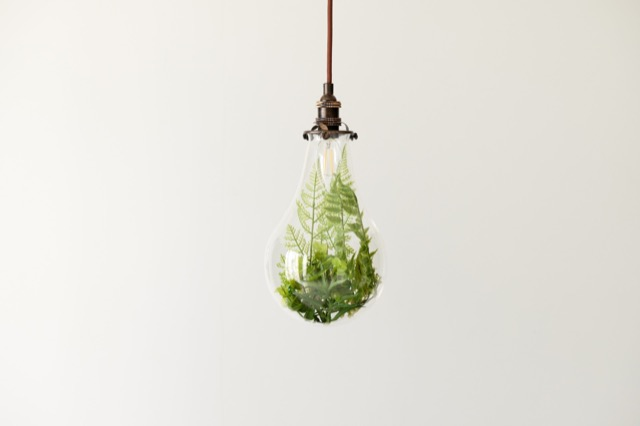
\includegraphics[height=3cm]{ex_155_img_1.png}
        \caption{[a lightbulb] surrounding [some plants]}
        \end{subfigure}%
        \caption*{\textit{Object}}
    \end{minipage}
    \hfill
    \begin{minipage}[t]{.30\textwidth}
        \begin{subfigure}[t]{\textwidth}
        \centering
        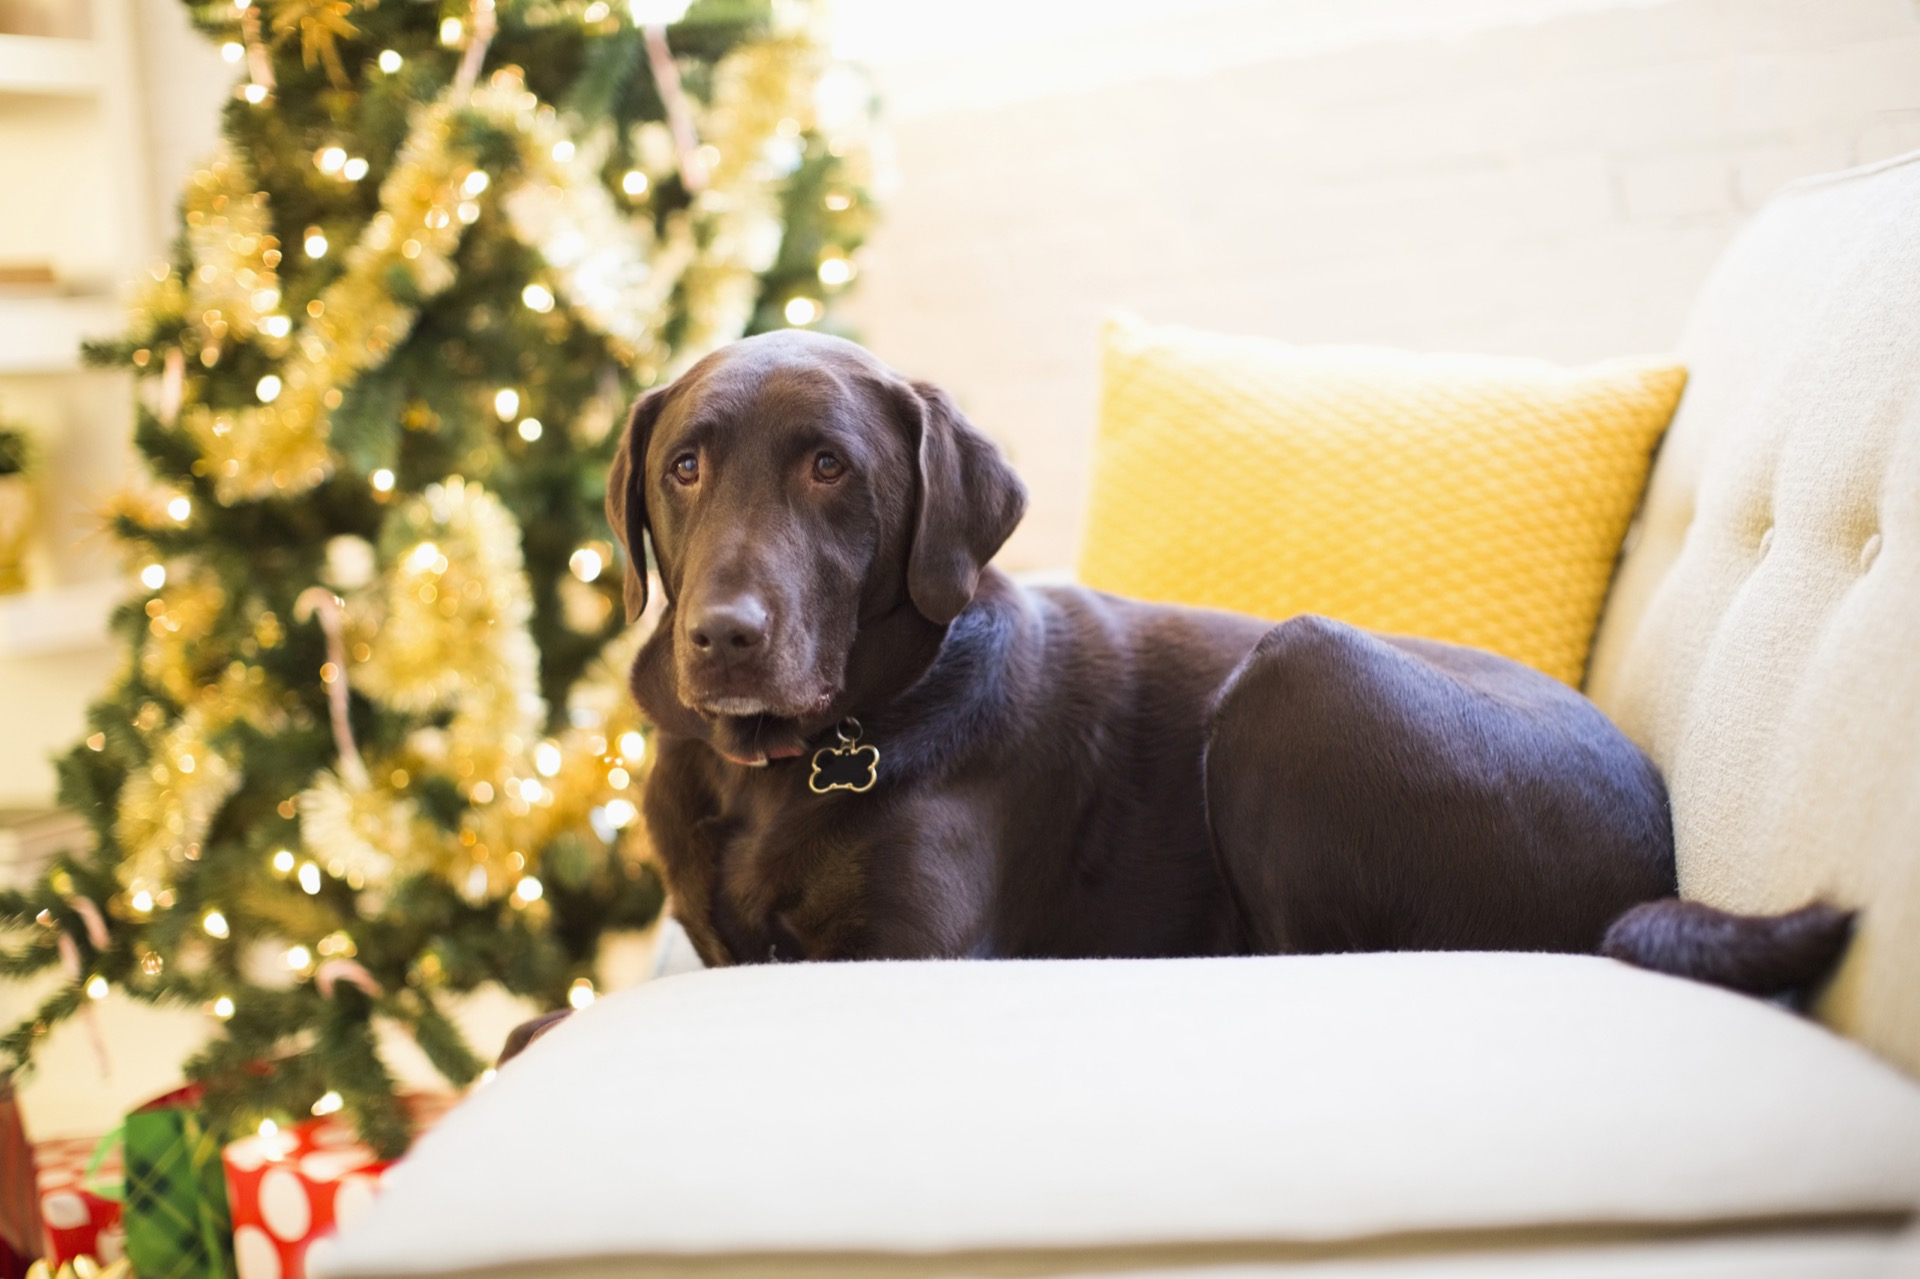
\includegraphics[height=3cm]{ex_29_img_0.png}
        \caption{a [brown] dog is on a [white] couch}
        \end{subfigure}\\
        \vspace{10pt}
        \begin{subfigure}[t]{\textwidth}
        \centering
        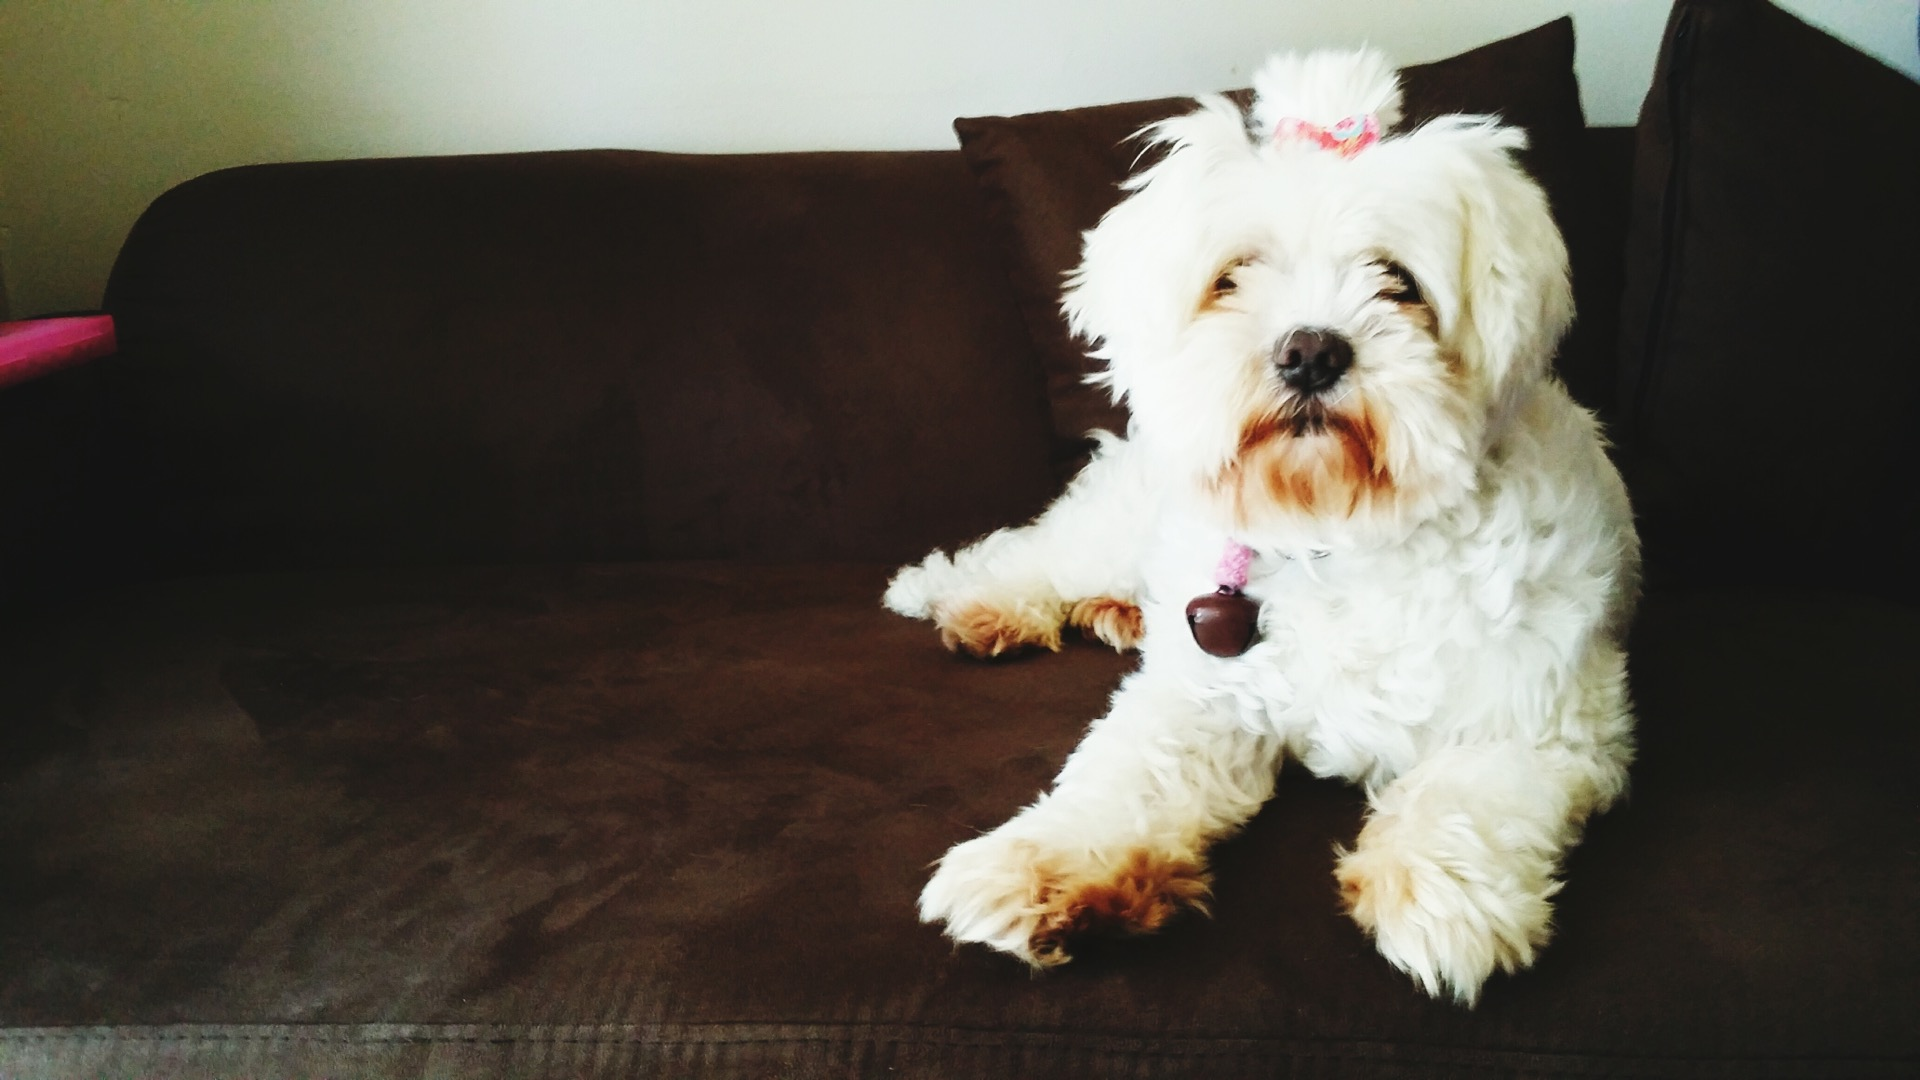
\includegraphics[height=3cm]{ex_29_img_1.png}
        \caption{a [white] dog is on a [brown] couch}
        \end{subfigure}% 
        \vspace{10pt}
        \caption*{\textit{Relation}}
    \end{minipage}
    \hfill
    \begin{minipage}[t]{.30\textwidth}
        \begin{subfigure}[t]{\textwidth}
        \centering
        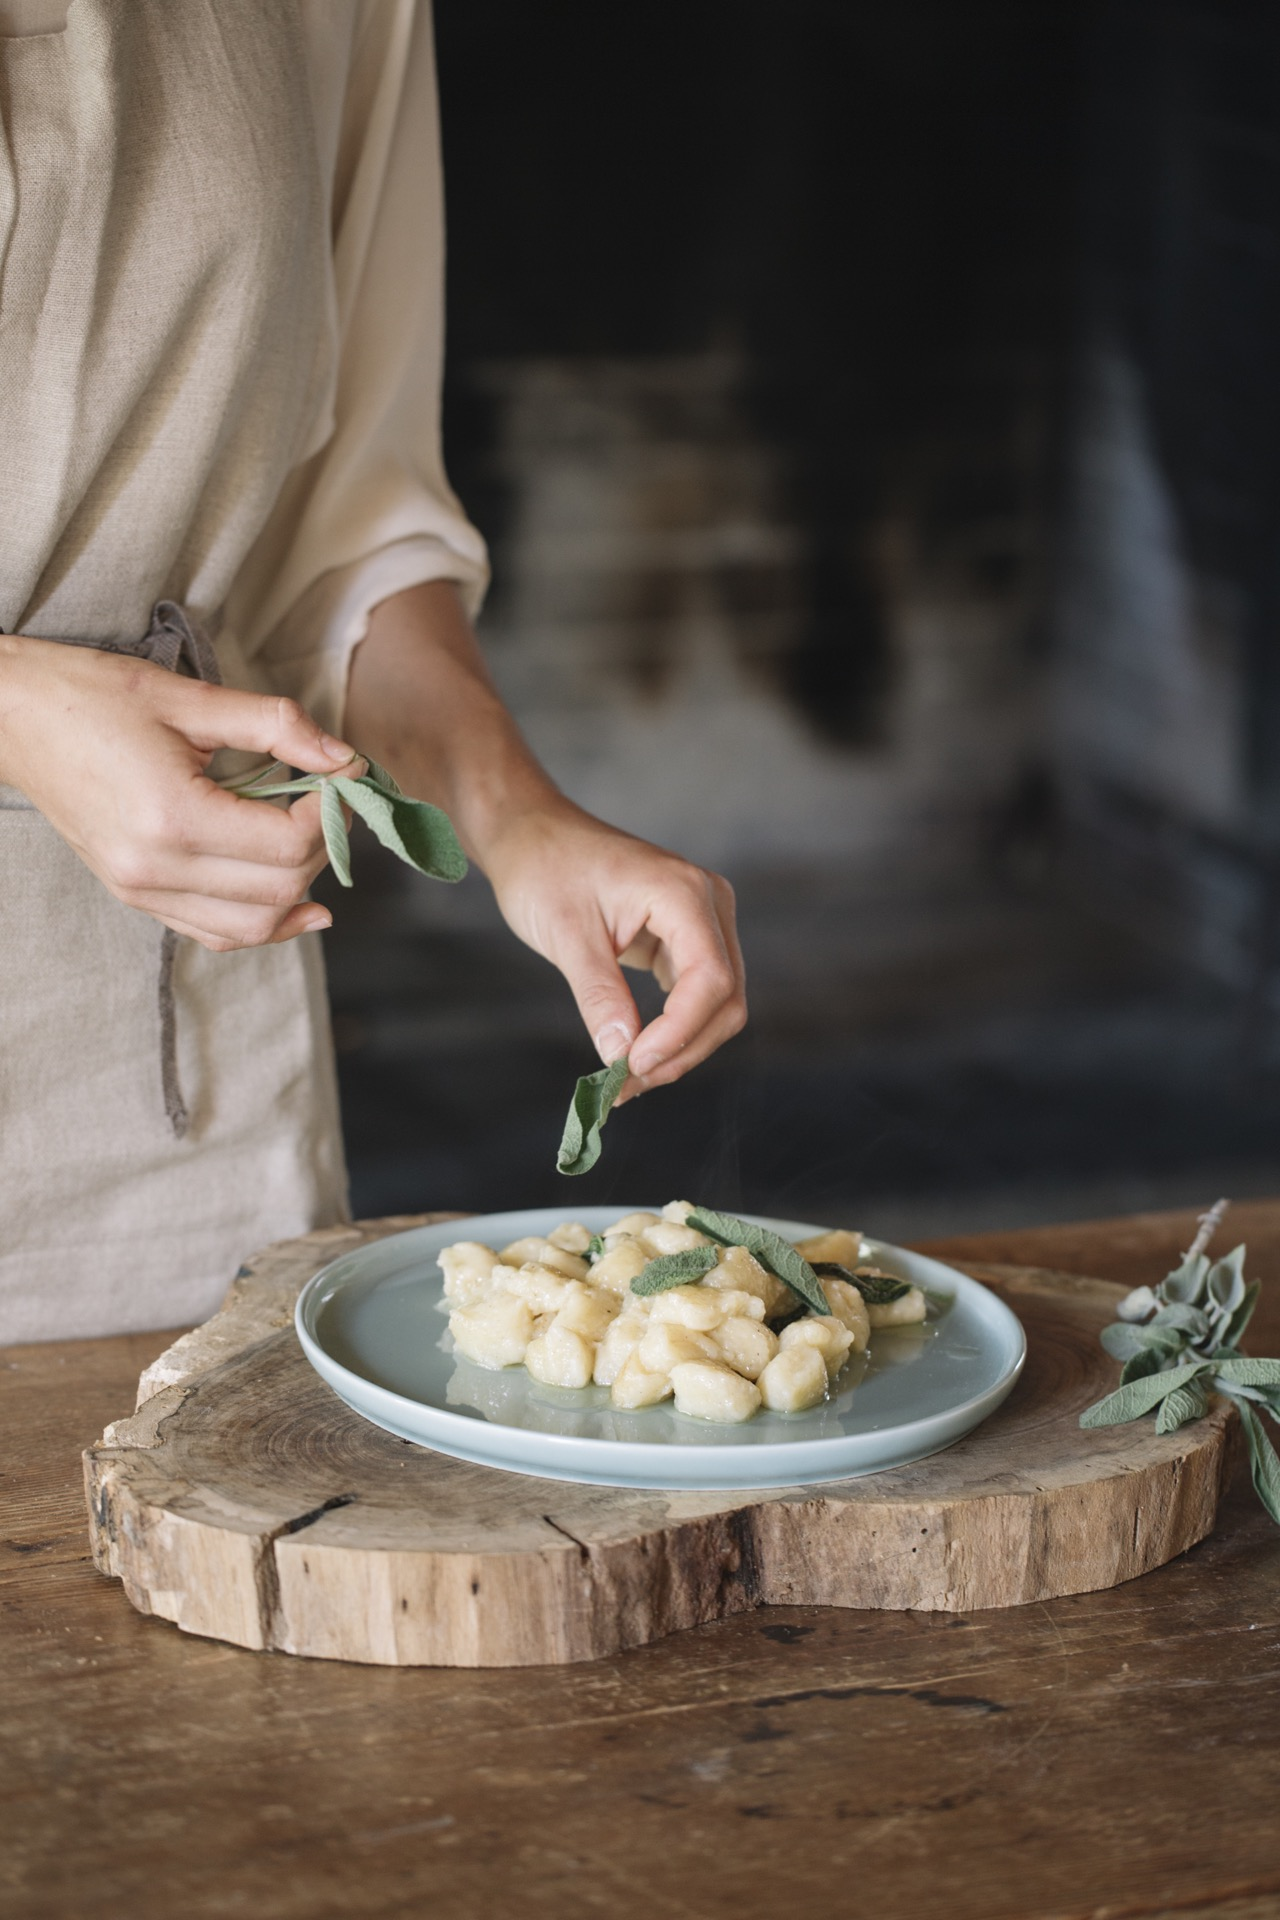
\includegraphics[height=3cm]{ex_118_img_0.png}
        \caption{[circular] food on [heart-shaped] wood}
        \end{subfigure}\\
        \begin{subfigure}[t]{\textwidth}
        \centering
        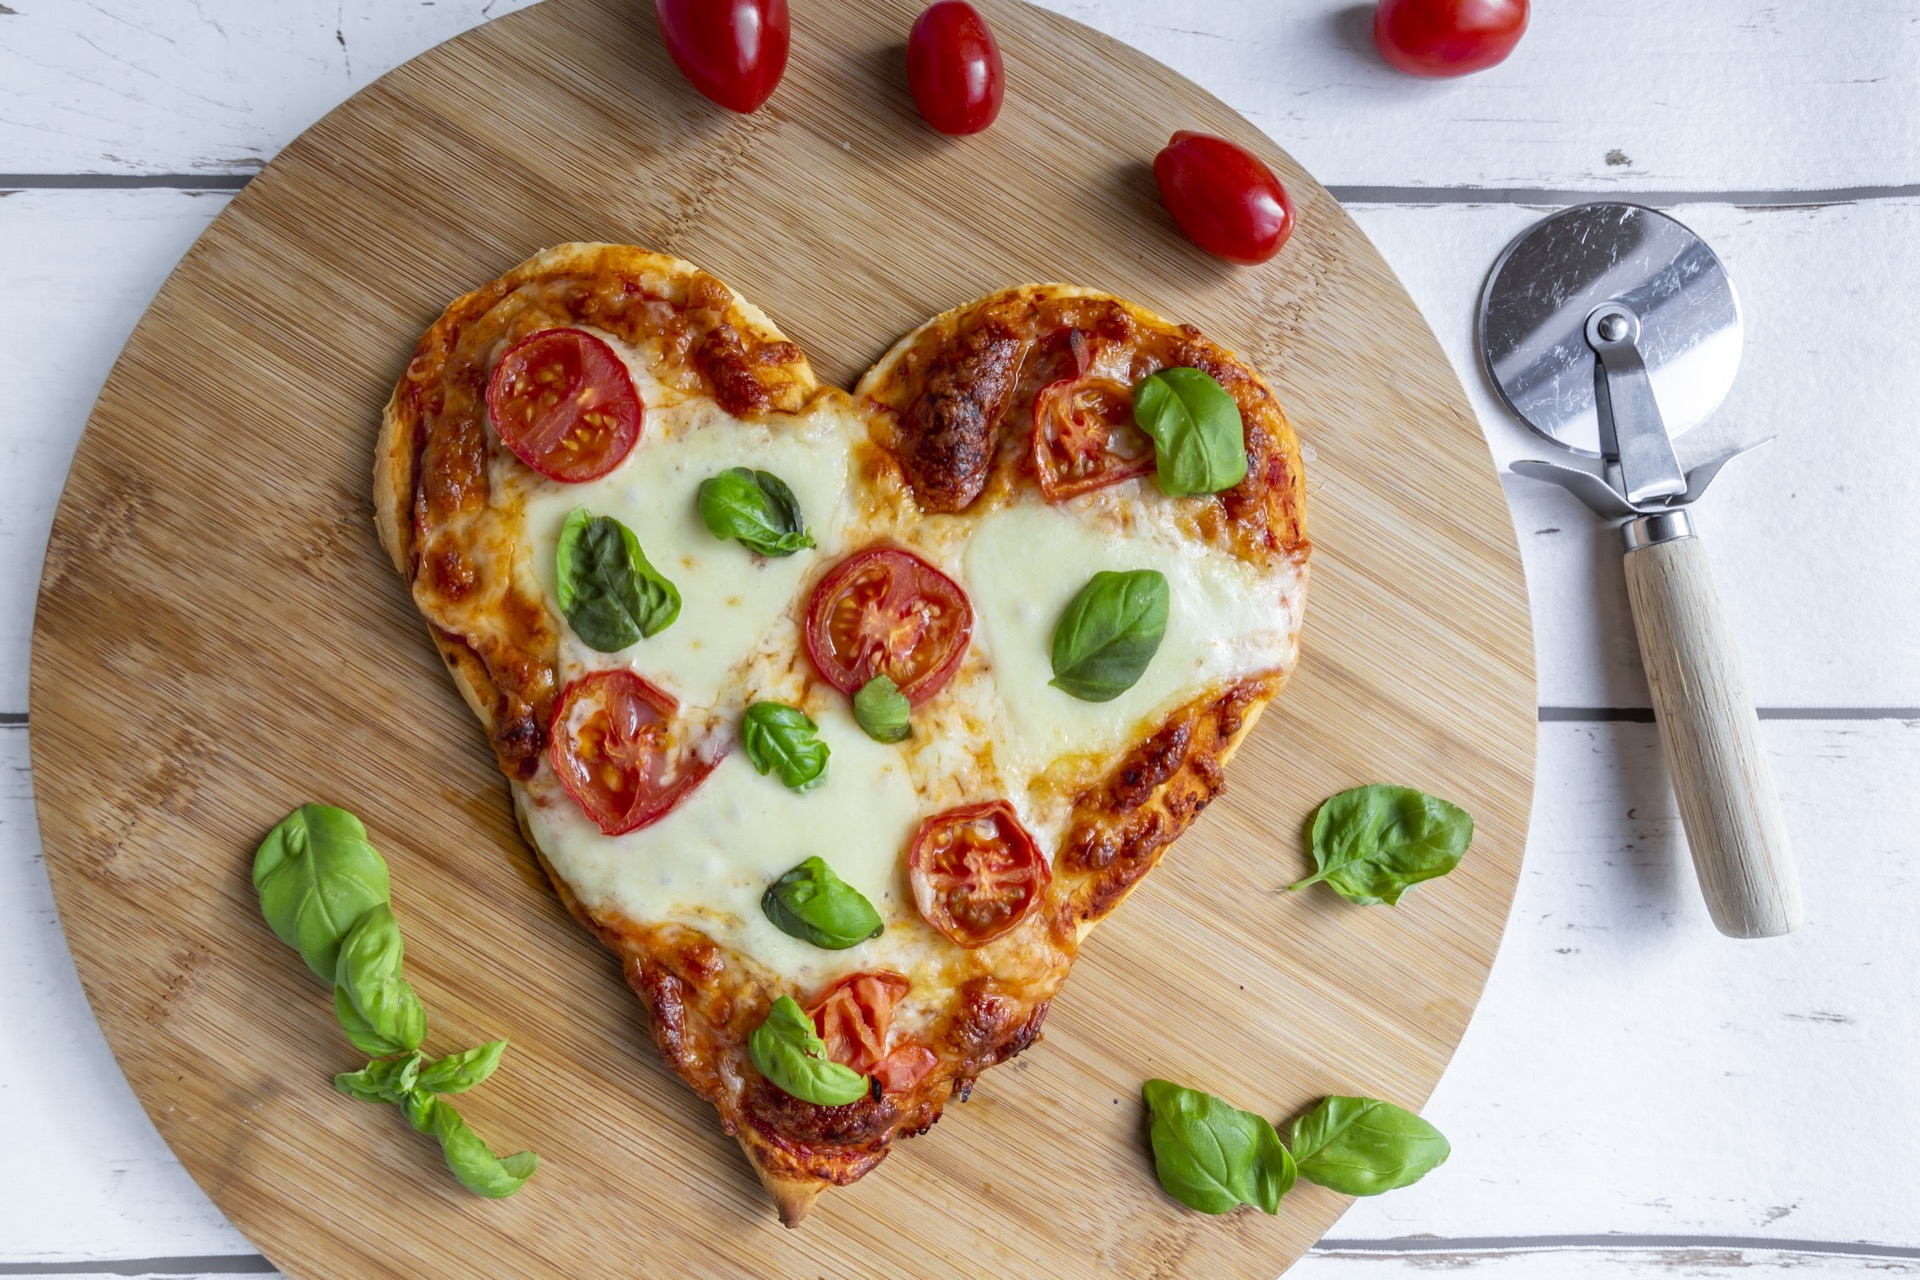
\includegraphics[height=3cm]{ex_118_img_1.png}
        \caption{[heart-shaped] food on [circular] wood}
        \end{subfigure}%
        \caption*{\textit{Relation}}
    \end{minipage}%
    \caption{Examples from the Winoground dataset for the swap-dependent linguistic tags \textit{Object}, \textit{Relation} and \textit{Relation} from left to right. They are additionally tagged with 1 main predicate.}
    \label{fig:winoground-examples}
\end{figure}

\begin{figure}[ht]
\centering
    \begin{minipage}[t]{.30\textwidth}
        \begin{subfigure}[t]{\textwidth}
        \centering
        
\includegraphics[height=3cm]{ex_14_img_0.png}
        \caption{there is [a mug] in [some grass]}
        \end{subfigure}\\
        \begin{subfigure}[t]{\textwidth}
        \centering
        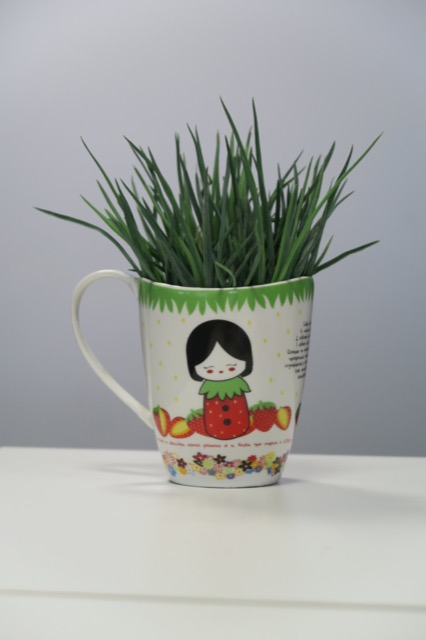
\includegraphics[height=3cm]{ex_14_img_1.png}
        \caption{there is [some grass] in [a mug]}
        \end{subfigure}%    
        \caption*{\textit{Object}}
    \end{minipage}
    \hfill
    \begin{minipage}[t]{.30\textwidth}
        \begin{subfigure}[t]{\textwidth}
        \centering
        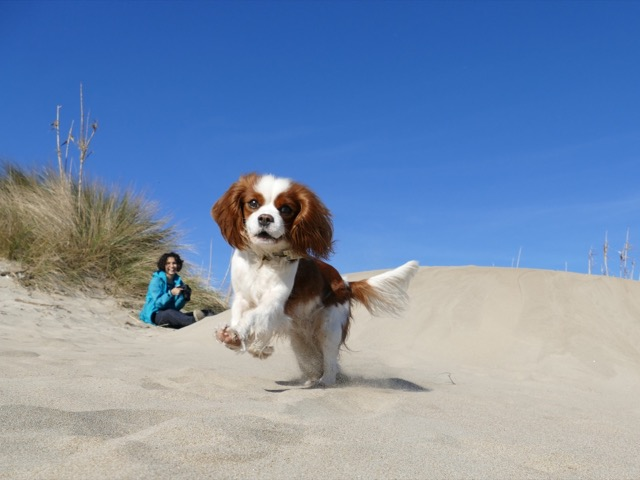
\includegraphics[height=3cm]{ex_21_img_0.png}
        \caption{a person [sits] and a dog [stands]}
        \end{subfigure}\\
        \begin{subfigure}[t]{\textwidth}
        \centering
        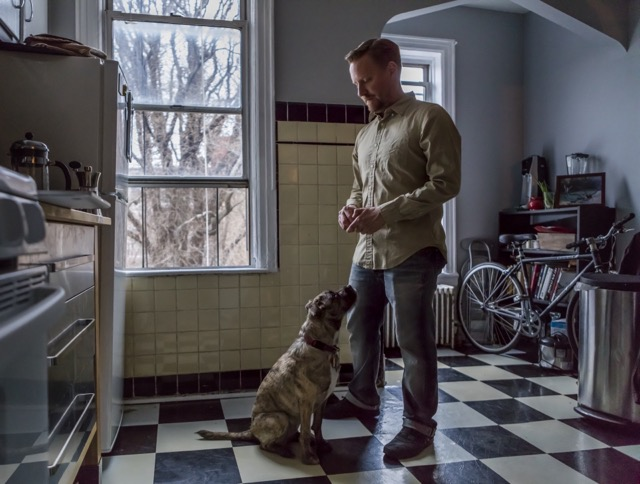
\includegraphics[height=3cm]{ex_21_img_1.png}
        \caption{a person [stands] and a dog [sits]}
        \end{subfigure}%    
        \caption*{\textit{Relation}}
    \end{minipage}
    \hfill
    \begin{minipage}[t]{.30\textwidth}
        \begin{subfigure}[t]{\textwidth}
        \centering
        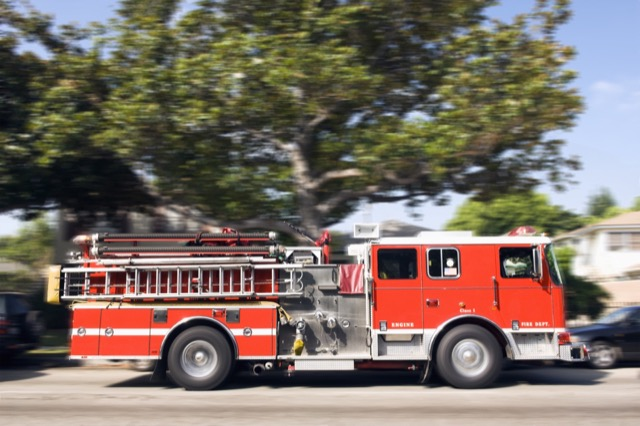
\includegraphics[height=3cm]{ex_72_img_0.png}
        \caption{it's a [fire] [truck]}
        \end{subfigure}\\
        \begin{subfigure}[t]{\textwidth}
        \centering
        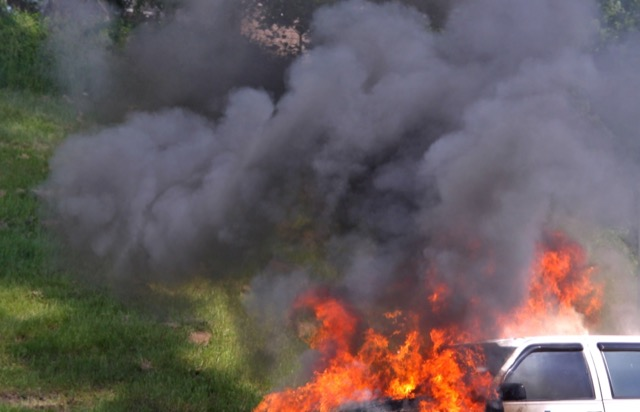
\includegraphics[height=3cm]{ex_72_img_1.png}
        \caption{it's a [truck] [fire]}
        \end{subfigure}%
        \caption*{\textit{Both}}
    \end{minipage}%
    \caption{Examples from the Winoground dataset for the swap-dependent linguistic tags \textit{Object}, \textit{Relation} and \textit{Both} from left to right. They are additionally tagged with 1, 2 and 1 main predicates from left to right.}
    \label{fig:winoground-examples-linguistic}
\end{figure}

On the other hand, there are three non-mutually exclusive \textbf{visual reasoning tags}: Pragmatics, Series and Symbolic. \textbf{Pragmatics} tag includes images that need to be interpreted non-literally. \textbf{Series} tag contains examples where both images come from the same photo series. \textbf{Symbolic} tag represents that the images include a symbolic representation. \cref{fig:winoground-examples-visual} shows examples of visual tags.

\begin{figure}[ht]
\centering
    \begin{minipage}{.30\textwidth}
        \begin{subfigure}{\textwidth}
        \centering
        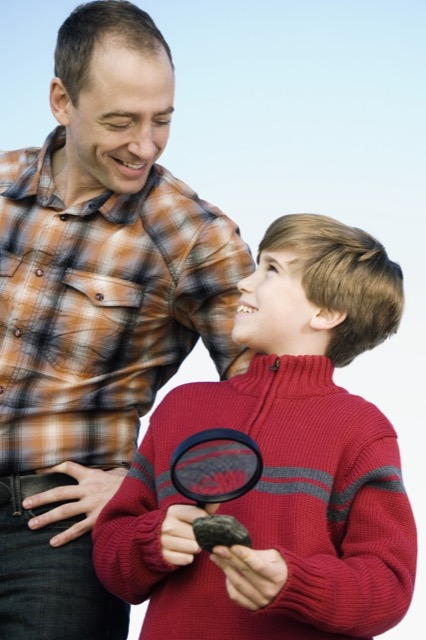
\includegraphics[height=3cm]{ex_75_img_0.png}
        \caption{the kid [with the magnifying glass] looks at them []}
        \end{subfigure}\\
        \begin{subfigure}{\textwidth}
        \centering
        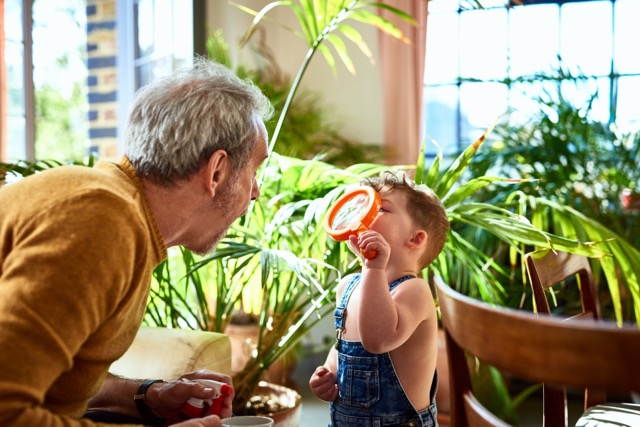
\includegraphics[height=3cm]{ex_75_img_1.png}
        \caption{the kid [] looks at them [with the magnifying glass]}
        \end{subfigure}%    
        \caption*{\textit{Pragmatics}}
    \end{minipage}
    \hfill
    \begin{minipage}{.30\textwidth}
        \begin{subfigure}{\textwidth}
        \centering
        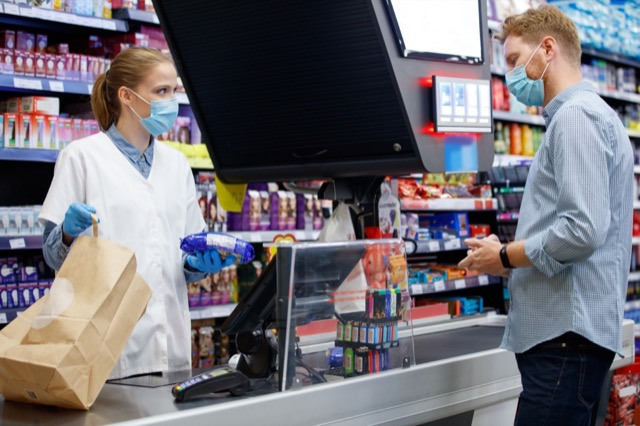
\includegraphics[height=3cm]{ex_27_img_0.png}
        \caption{the person with the ponytail [packs] stuff and other [buys] it}
        \end{subfigure}\\
        \begin{subfigure}{\textwidth}
        \centering
        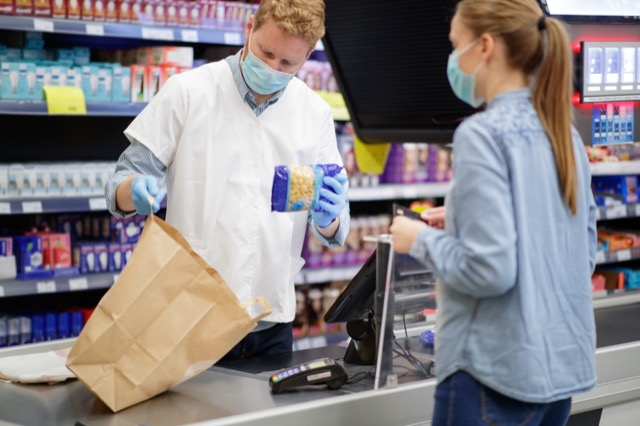
\includegraphics[height=3cm]{ex_27_img_1.png}
        \caption{the person with the ponytail [buys] stuff and other [packs] it}
        \end{subfigure}%    
        \caption*{\textit{Series}}
    \end{minipage}
    \hfill
    \begin{minipage}{.30\textwidth}
        \begin{subfigure}{\textwidth}
        \centering
        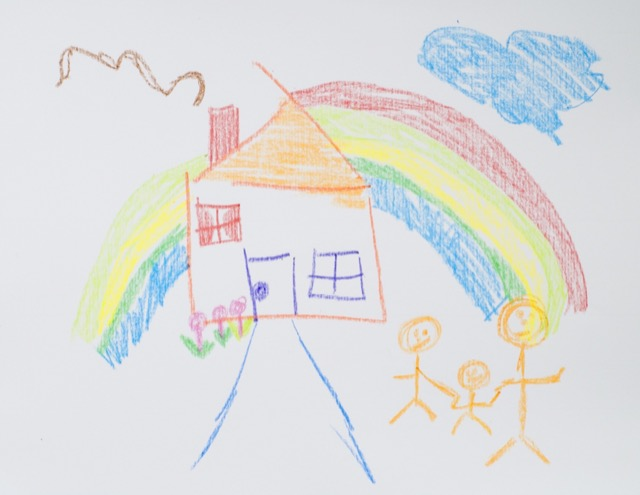
\includegraphics[height=3cm]{ex_61_img_0.png}
        \caption{there are [three] people and [two] windows}
        \end{subfigure}\\
        \begin{subfigure}{\textwidth}
        \centering
        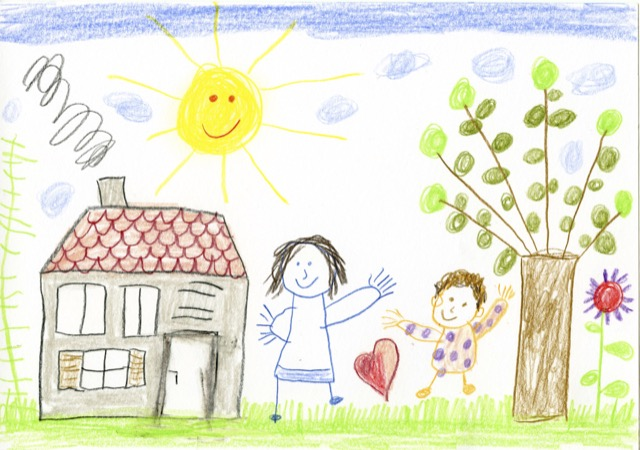
\includegraphics[height=3cm]{ex_61_img_1.png}
        \caption{there are [two] people and [three] windows}
        \end{subfigure}%    
        \caption*{\textit{Symbolic}}
    \end{minipage}
    \caption{Examples from the Winoground dataset for the visual tags \textit{Pragmatics}, \textit{Series} and \textit{Symbolic} from left to right. They are additionally tagged with the \textit{Relation} tag, and 1, 2, and 1 main predicates from left to right.}
    \label{fig:winoground-examples-visual}
\end{figure}

\subsection{Metrics}

\paragraph{Score.}
Performance on Winoground \cite{thrush2022winoground} is computed according to three different metrics that evaluate different aspects of the models' visio-linguistic reasoning abilities.

The first metric is the \textbf{text score}, which measures whether a model can select the correct caption, given an image. 
Given images $I_0$ and $I_{1}$ and captions $C_{0}$ and $C_{1}$, the text score for an example $(C_{0},I_{0},C_{1},I_{1})$ is computed according to:
\begin{equation}\label{eq:text-score}
        ts(C_{0},I_{0},C_{1},I_{1})= 
    \begin{cases}
        1 & \text{if}\  s(C_{0}, I_{0}) > s(C_{1}, I_{0}) \\
        & \ \ \text{and}\ s(C_{1}, I_{1}) > s(C_{0}, I_{1}) \\
        0              & \text{otherwise}
    \end{cases}
\end{equation}
where $s(\cdot)$ is the model's score for the image/caption pair.

The second metric is the \textbf{image score}, which measures whether a model can select the correct image, given a caption.
The image score for an example is computed according to:
\begin{equation}\label{eq:image-score}
        is(C_{0},I_{0},C_{1},I_{1})= 
    \begin{cases}
        1 & \text{if}\  s(C_{0}, I_{0}) > s(C_{0}, I_{1})\\
        & \ \ \text{and}\ s(C_{1}, I_{1}) > s(C_{1}, I_{0}) \\
        0              & \text{otherwise}
    \end{cases}
\end{equation}

Our final metric \textbf{group score} combines the previous two, which measures if every combination for a given example is correctly scored by the model.
The group score for an example is computed according to:
\begin{equation}\label{eq:group-score}
        gs(C_{0},I_{0},C_{1},I_{1})= 
    \begin{cases}
        1 & \text{if}\  ts(C_{0},I_{0},C_{1},I_{1})  \\
         & \ \ \text{and}\ is(C_{0},I_{0},C_{1},I_{1})\\
        0              & \text{otherwise}
    \end{cases}
\end{equation}

\paragraph{Accuracy.}
We also add three additional accuracy metrics. These are similar to the previous ones, but accuracy is 0.5 when one of the pairs is correct.

Given images $I_0$ and $I_{1}$ and captions $C_{0}$ and $C_{1}$, the \textbf{text accuracy} for an example $(C_{0},I_{0},C_{1},I_{1})$ is computed according to:
\begin{equation}\label{eq:text-accuracy}
        ta(C_{0},I_{0},C_{1},I_{1})= 
    \begin{cases}
        1 & \text{if}\  s(C_{0}, I_{0}) > s(C_{1}, I_{0}) \\
        & \ \ \text{and}\ s(C_{1}, I_{1}) > s(C_{0}, I_{1}) \\
        0.5 & \text{if}\  s(C_{0}, I_{0}) > s(C_{1}, I_{0}) \\
        & \ \ \text{xor}\ s(C_{1}, I_{1}) > s(C_{0}, I_{1}) \\
        0              & \text{otherwise}
    \end{cases}
\end{equation}
where $s(\cdot)$ is the model's score for the image/caption pair.

The \textbf{image accuracy} for an example is computed according to:
\begin{equation}\label{eq:image-accuracy}
        ia(C_{0},I_{0},C_{1},I_{1})= 
    \begin{cases}
        1 & \text{if}\  s(C_{0}, I_{0}) > s(C_{0}, I_{1})\\
        & \ \ \text{and}\ s(C_{1}, I_{1}) > s(C_{1}, I_{0}) \\
        0.5 & \text{if}\  s(C_{0}, I_{0}) > s(C_{0}, I_{1})\\
        & \ \ \text{xor}\ s(C_{1}, I_{1}) > s(C_{1}, I_{0}) \\
        0              & \text{otherwise}
    \end{cases}
\end{equation}

The \textbf{group accuracy} in our framework is computed according to:
\begin{equation}\label{eq:group-accuracy}
        ga(C_{0},I_{0},C_{1},I_{1})= 
        (ta(C_{0},I_{0},C_{1},I_{1}) + ia(C_{0},I_{0},C_{1},I_{1})) / 2\\
\end{equation}

\section{Visual Spatial Reasoning} \label{sec:vsr}

This section describes the Visual Spatial Reasoning (VSR) \cite{liu2022visual} dataset and the splits that are used for evaluation.

\subsection{Dataset}

The objective of VSR is to \textbf{test spatial grounding} capabilities by covering \textbf{65 spatial relations} over natural images from COCO. Given an image and a caption which describes a spatial relation between two of the objects, the model has to infer if the relation is true or false.

A \textbf{contrastive caption generation} approach was used in VSR to avoid choosing too many trivial relations. First, a pair of images that contain the same two concepts are selected from COCO. Second, an annotator had to choose a spatial relation that made the caption template correct for one image but incorrect for the other. Finally, every item is reviewed by at least two additional human annotators. If the agreement between annotators is not high enough, the data point is excluded.

To get a more high-level understanding of the relations, they are grouped in \textbf{meta categories} \cite{marchi2021cross}: Adjacency, Directional, Orientation, Projective, Proximity, Topological and Unallocated (see \cref{tab:spatial_relations}). We show some examples to understand the differences between relation categories in Figures \ref{fig:vsr-examples} and \ref{fig:vsr-examples-2}.

\begin{table}[ht]
    \centering
    \begin{adjustbox}{max width=\textwidth}
    \begin{tabular}{l|l}
    \toprule
        \rowcolor{DarkGray}
    Category & Spatial Relations \\
    \midrule
    Adjacency   & \makecell[l]{Adjacent to, alongside, at the side of, at the right side of, at the left side of, attached to, at the back of,\\ ahead of, against, at the edge of} \\
    \rowcolor{Gray}
 Directional & \makecell[l]{Off, past, toward, down, deep down$^\ast$, up$^\ast$, away from, along, around, from$^\ast$, into, to$^\ast$, across, across from, \\through$^\ast$, down from }\\
    Orientation & Facing, facing away from, parallel to, perpendicular to\\
    \rowcolor{Gray}
    Projective & On top of, beneath, beside, behind, left of, right of, under, in front of, below, above, over, in the middle of\\
    Proximity & By, close to, near, far from, far away from \\
        \rowcolor{Gray}
    Topological & \makecell[l]{Connected to, detached from, has as a part, part of, contains, within, at, on, in, with, surrounding, among, \\ consists of, out of, between, inside, outside, touching}\\
    Unallocated & Beyond, next to, opposite to, after$^\ast$, among, enclosed by \\
\bottomrule
    \end{tabular}
    \end{adjustbox}
    \caption{The available 71 spatial relations. 65 of them appear in the final dataset. Relations with $\ast$ are not used.}
    % unused: 'up', 'through', 'deep down', 'from', 'to', 'after'
    \label{tab:spatial_relations}
\end{table}

In \cref{fig:vsr-examples} we show examples of Adjacency, Projective and Topological meta categories. \textbf{Adjacency} examples involve identifying what is ahead of the cow and which is the edge of the table. The \textbf{Projective} images are paired with the same caption, but have different labels. \textbf{Topological} examples require understanding what being inside and touching are.

\begin{figure}[ht]
\centering
    \begin{minipage}[t]{.30\textwidth}
        \begin{subfigure}[t]{\textwidth}
        \centering
        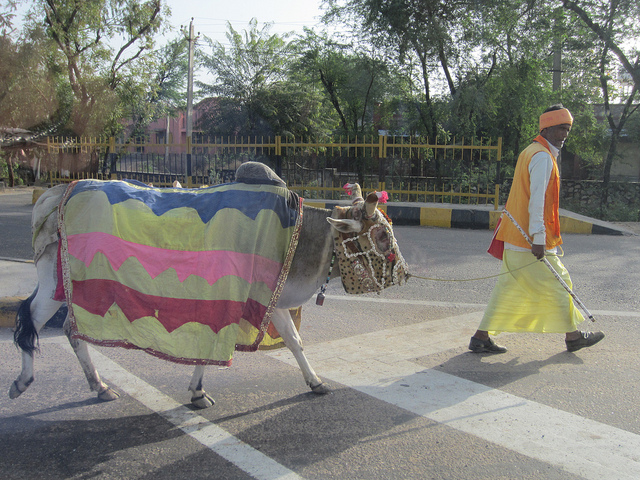
\includegraphics[height=3cm]{000000080336.jpg}
        \caption{Caption: \textit{The person is ahead of the cow.} Label: \texttt{True}.}
        \label{fig:person_cow}
        \end{subfigure}\\
        \begin{subfigure}[t]{\textwidth}
        \centering
        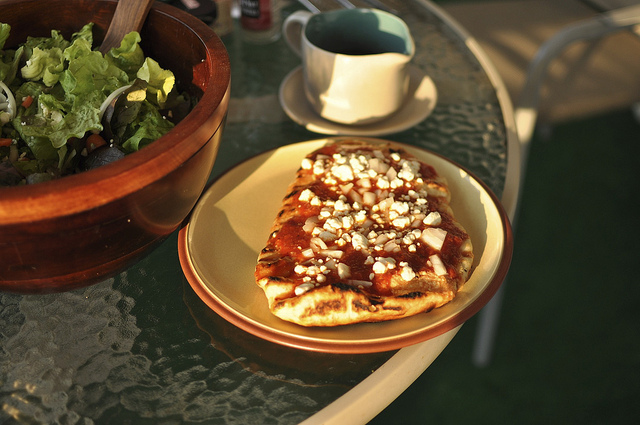
\includegraphics[height=3cm]{000000261511.jpg}
        \caption{Caption: \textit{The pizza is at the edge of the dining table.} Label: \texttt{True}.}
        \label{fig:pizza_table}
        \end{subfigure}%
        \caption*{\textit{Adjacency}}
    \end{minipage}
    \hfill
    \begin{minipage}[t]{.30\textwidth}
        \begin{subfigure}[t]{\textwidth}
        \centering
        
\includegraphics[height=3cm]{000000119360.jpg}
        \caption{Caption: \textit{The cat is behind the laptop.} Label: \texttt{True}.}
        \end{subfigure}\\
        \begin{subfigure}[t]{\textwidth}
        \centering
        
\includegraphics[height=3cm]{000000310958.jpg}
        \caption{Caption: \textit{The cat is behind the laptop.} Label: \texttt{False}.}
        \end{subfigure}% 
        \caption*{\textit{Projective}}
    \end{minipage}
    \hfill
    \begin{minipage}[t]{.30\textwidth}
        \begin{subfigure}[t]{\textwidth}
        \centering
        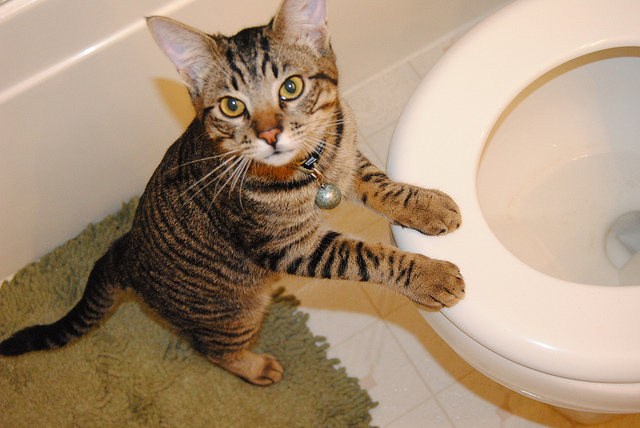
\includegraphics[height=3cm]{000000292365.jpg}
        \caption{Caption: \textit{The cat is inside the toilet.} Label: \texttt{False}.}
        \label{fig:cat_toilet_true}
        \end{subfigure}\\
        \begin{subfigure}[t]{\textwidth}
        \centering
        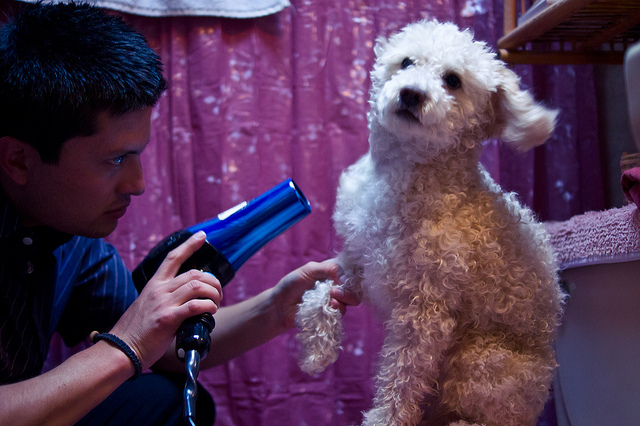
\includegraphics[height=3cm]{000000092020.jpg}
        \caption{Caption: \textit{The person is touching the hair drier.} Label: \texttt{True}.}
        \label{fig:cat_toilet}
        \end{subfigure}%
        \caption*{\textit{Topological}}
    \end{minipage}%
    \caption{Examples from the VSR dataset for the relation meta categories \textit{Adjacency}, \textit{Projective} and \textit{Topological} from left to right.}
    \label{fig:vsr-examples}
\end{figure}

In \cref{fig:vsr-examples-2} Adjacency, Projective and Orientation meta categories. The first \textbf{Adjacency} example is tricky, it requires knowing which is the right side of the bench. The second one is even more difficult because the cow both the cow appears in the car’s side mirror. \textbf{Projective} examples involve knowing where is the front of the person and below the cat. \textbf{Orientation} examples require understanding the orientations of the hair drier and the fire hydrant.

\begin{figure}[ht]
\centering
    \begin{minipage}[t]{.30\textwidth}
        \begin{subfigure}[t]{\textwidth}
        \centering
        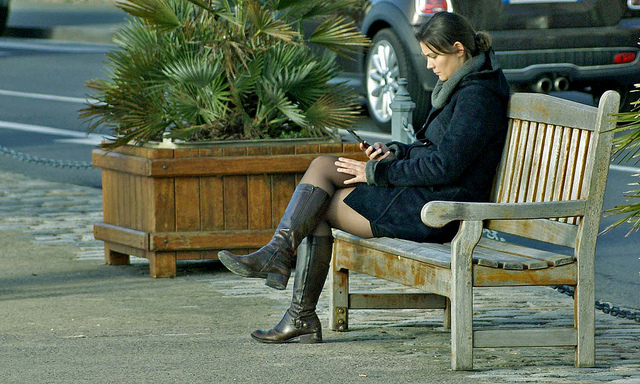
\includegraphics[height=3cm]{000000259555.jpg}
        \caption{Caption: \textit{The potted plant is at the right side of the bench.} Label: \texttt{True}.}
        \end{subfigure}\\
        \begin{subfigure}[t]{\textwidth}
        \centering
        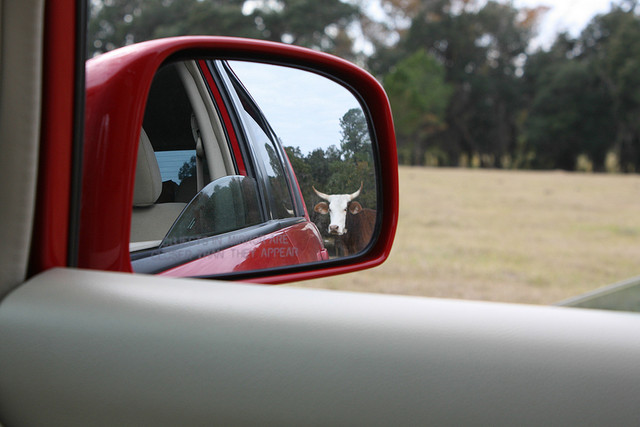
\includegraphics[height=3cm]{000000512796.jpg}
        \caption{Caption: \textit{The cow is at the back of the car.} Label: \texttt{True}.}
        \end{subfigure}%
        \caption*{\textit{Adjacency}}
    \end{minipage}
    \hfill
    \begin{minipage}[t]{.30\textwidth}
        \begin{subfigure}[t]{\textwidth}
        \centering
        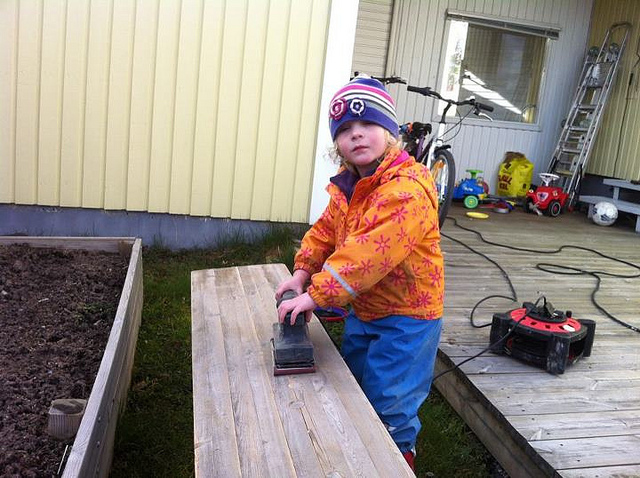
\includegraphics[height=3cm]{000000434410.jpg}
        \caption{Caption: \textit{The bench is in front of the person.} Label: \texttt{True}.}
        \end{subfigure}\\
        \begin{subfigure}[t]{\textwidth}
        \centering
        
\includegraphics[height=3cm]{000000420344.jpg}
        \caption{Caption: \textit{The keyboard is below the cat.} Label: \texttt{True}.}
        \end{subfigure}%
        \caption*{\textit{Projective}}
    \end{minipage}
    \hfill
    \begin{minipage}[t]{.30\textwidth}
        \begin{subfigure}[t]{\textwidth}
        \centering
        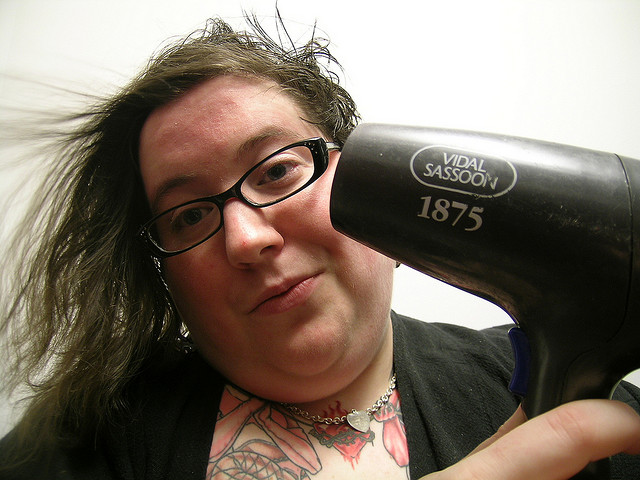
\includegraphics[height=3cm]{000000134738.jpg}
        \caption{Caption: \textit{The hair drier is facing away from the person.} Label: \texttt{False}.}
        \end{subfigure}\\
        \begin{subfigure}[t]{\textwidth}
        \centering
        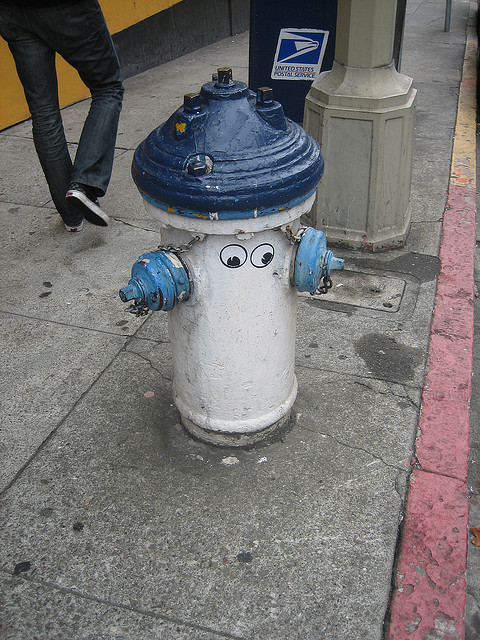
\includegraphics[height=3cm]{000000147270.jpg}
        \caption{Caption: \textit{The fire hydrant is facing away from the person.} Label: \texttt{True}.}
        \end{subfigure}% 
        \caption*{\textit{Orientation}}
    \end{minipage}%
    \caption{Examples from the VSR dataset for the relation meta categories \textit{Adjacency}, \textit{Projective} and \textit{Orientation} from left to right.}
    \label{fig:vsr-examples-2}
\end{figure}

\subsection{Dataset Splits}\label{sec:vsr_splits}

The VSR dataset has two types of splits \cite{liu2022visual}, random and zero-shot. The statistics of the two splits are shown in \cref{tab:data_splits}.

\begin{table}[ht]
\small
\centering
\begin{tabular}{lllll}
\toprule
 split & train & dev & test & total   \\
\midrule
\textit{random} & 7,083 & 1,012 & 2,024 & 10,119 \\
\textit{zero-shot} & 5,440 & 259 & 731  & 6,430\\
\bottomrule
\end{tabular}
\caption{Data statistics of the \textit{random} and \textit{zero-shot} splits. }
\label{tab:data_splits}
\end{table}

\paragraph{Random split.}
The dataset is split randomly into train/dev/test with the ratio of 70\%/10\%/20\%. All the validated data points are used in this split.

\paragraph{Zero-shot split.}
It is a concept zero-shot split where train/dev/test have no overlapping concepts. That is, each concept can only appear in one of the sets.
This is done by randomly grouping concepts into three sets with the ratio of 50\%/20\%/30\%.
This is a more challenging setup because the model has to learn concepts and relations in a compositional way instead of remembering the co-occurrence of the two.
Moreover, having less training data is a disadvantage for the models, since not all the data can be used in this setting.